\documentclass[tikz,border=10pt]{standalone}
\usepackage{tikz}
\usetikzlibrary{positioning,shapes,arrows.meta}

\begin{document}
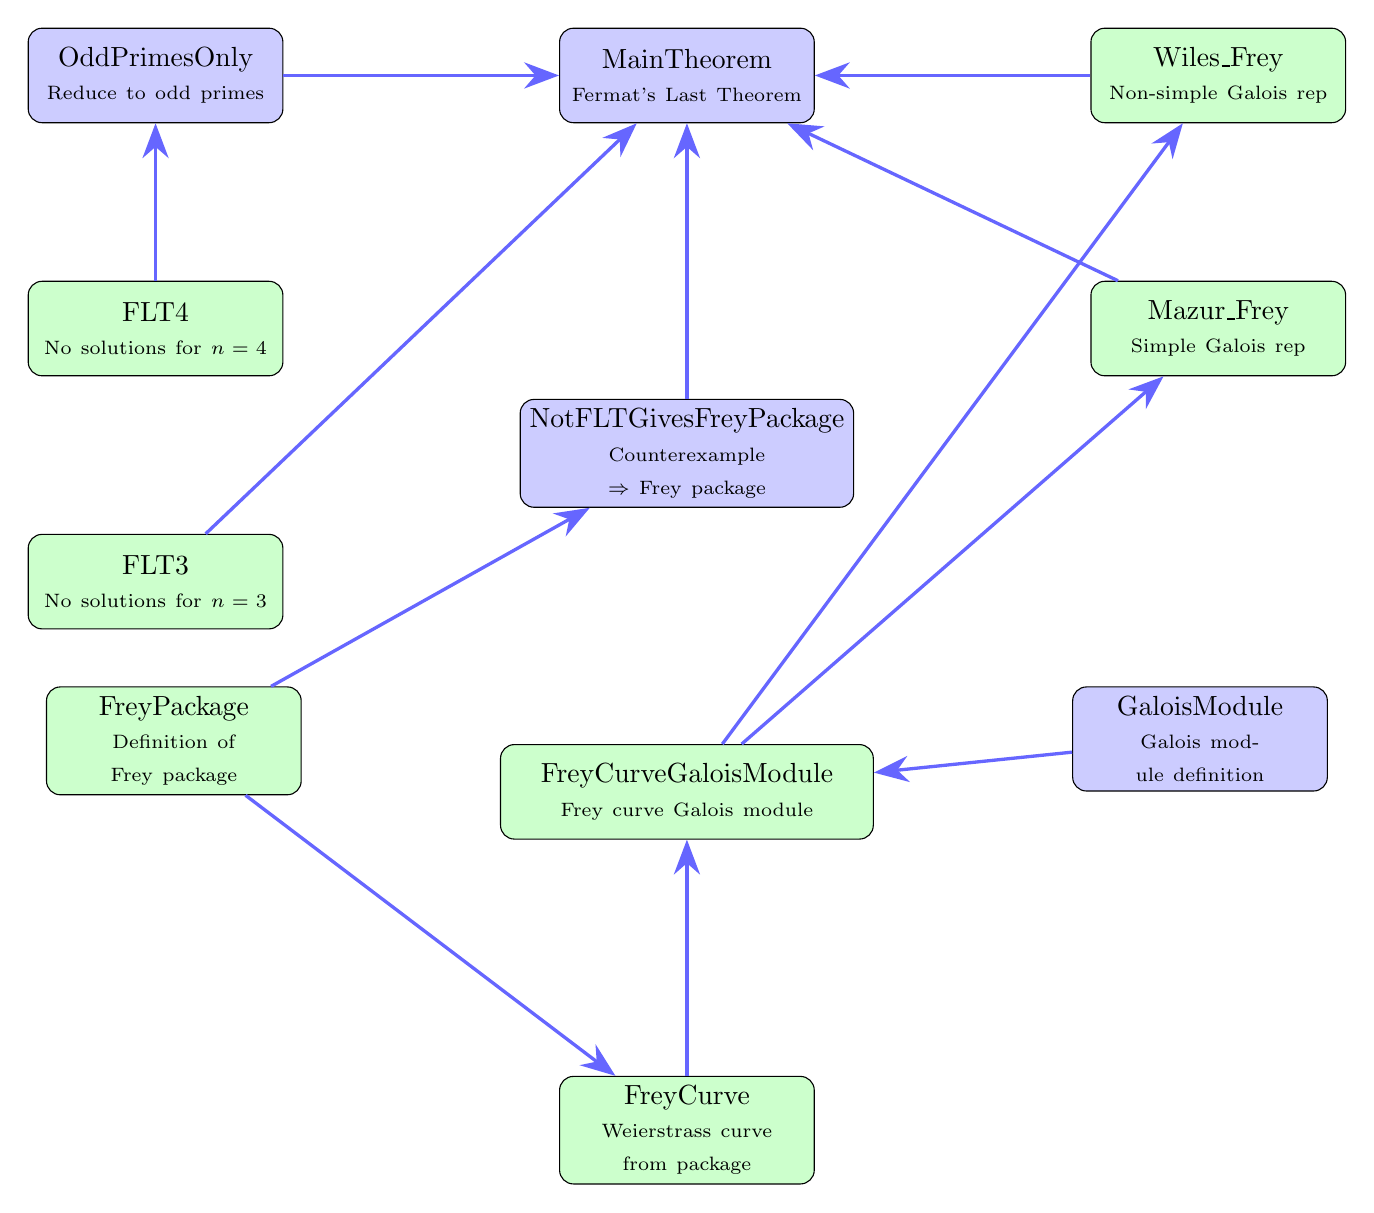
\begin{tikzpicture}[
    node distance=2.5cm,
    every node/.style={
        draw,
        rounded corners=5pt,
        text width=3cm,
        text centered,
        minimum height=1.2cm,
        font=\normalsize
    },
    hypothesis/.style={fill=green!20},
    theorem/.style={fill=blue!20},
    definition/.style={fill=blue!20},
    arrow/.style={-{Stealth[scale=1.5]}, very thick, color=blue!60}
]

% Main theorem at the top center
\node[theorem] (main) at (0,8) {MainTheorem\\{\scriptsize Fermat's Last Theorem}};

% Left side - upper level
\node[theorem, left=of main, xshift=-1cm] (odd) {OddPrimesOnly\\{\scriptsize Reduce to odd primes}};
\node[hypothesis, below=of odd, yshift=0.5cm] (flt4) {FLT4\\{\scriptsize No solutions for $n=4$}};
\node[hypothesis, below=of flt4, yshift=0.5cm] (flt3) {FLT3\\{\scriptsize No solutions for $n=3$}};

% Right side - upper level
\node[hypothesis, right=of main, xshift=1cm] (wiles) {Wiles\_Frey\\{\scriptsize Non-simple Galois rep}};
\node[hypothesis, below=of wiles, yshift=0.5cm] (mazur) {Mazur\_Frey\\{\scriptsize Simple Galois rep}};

% Middle-lower level
\node[theorem, below=of main, yshift=-1cm, text width=4cm] (notflt) {NotFLTGivesFreyPackage\\{\scriptsize Counterexample $\Rightarrow$ Frey package}};

% Bottom level
\node[hypothesis, below left=of notflt, xshift=-1cm, yshift=-0.5cm] (freypack) {FreyPackage\\{\scriptsize Definition of Frey package}};
\node[hypothesis, below=of notflt, yshift=-0.5cm, text width=4.5cm] (freygalois) {FreyCurveGaloisModule\\{\scriptsize Frey curve Galois module}};
\node[definition, below right=of notflt, xshift=1cm, yshift=-0.5cm] (galois) {GaloisModule\\{\scriptsize Galois module definition}};
\node[hypothesis, below=of freygalois, yshift=-0.5cm] (freycurve) {FreyCurve\\{\scriptsize Weierstrass curve from package}};

% Arrows showing dependencies
\draw[arrow] (odd) -- (main);
\draw[arrow] (flt3) -- (main);
\draw[arrow] (flt4) -- (odd);
\draw[arrow] (wiles) -- (main);
\draw[arrow] (mazur) -- (main);
\draw[arrow] (notflt) -- (main);
\draw[arrow] (freypack) -- (notflt);
\draw[arrow] (freypack) -- (freycurve);
\draw[arrow] (galois) -- (freygalois);
\draw[arrow] (freycurve) -- (freygalois);
\draw[arrow] (freygalois) -- (wiles);
\draw[arrow] (freygalois) -- (mazur);

\end{tikzpicture}
\end{document}